\RequirePackage{amsmath}
\documentclass[a4paper]{llncs}
\usepackage[utf8]{inputenc}
\PassOptionsToPackage{table}{xcolor}
\pagestyle{headings}  % This option shows page numbers, it have to be removed in the final document.
\usepackage{booktabs}
\usepackage{amssymb}
\usepackage{tikz}
\usepackage{scalerel}
\usepackage{comment}
\usepackage{framed}
\usepackage{listings}
\usepackage{mathtools}
%\usepackage{pifont}% http://ctan.org/pkg/pifont
%\usepackage{balance}
%\usepackage{stmaryrd}
\usepackage{adjustbox}
\usepackage{multirow}
\usepackage{enumitem}
\usepackage{xspace}
\usepackage{url}
\usepackage{inconsolata}
\usepackage{etoolbox}

\newcommand\copyrighttext{%
  \footnotesize Copyright © 2020 for this paper by its authors. Use permitted under Creative Commons License Attribution 4.0 International (CC BY 4.0).}
\newcommand\copyrightnotice{%
\begin{tikzpicture}[remember picture,overlay]
\node[anchor=south,yshift=70pt,xshift=\marginparsep] at (current page.south) {{\parbox{\dimexpr\textwidth-\fboxsep-\fboxrule\relax}{\copyrighttext}}};
\end{tikzpicture}%
}

\renewcommand{\UrlFont}{\ttfamily\scriptsize}

%%%%%%%%%%%%%%%%%%%%%%%%%%%%%%%%%%%%%%%%%%%%%%%%%%%%%%
%% Quickly switch from conference to extended version
\providetoggle{conf}
\settoggle{conf}{false}

% text only to appear in extended version
\newcommand{\ever}[1]{\iftoggle{conf}{}{#1}}

% text only to appear in the conference version
\newcommand{\cver}[1]{\iftoggle{conf}{#1}{}}

% alternate text for both versions
\newcommand{\cever}[2]{\iftoggle{conf}{#1}{#2}}

% environment for long extended-only text
\iftoggle{conf}%
 {\excludecomment{exver}}%
 {\newenvironment{exver}}%
%%%%%%%%%%%%%%%%%%%%%%%%%%%%%%%%%%%%%%%%%%%%%%%%%%%%%% 


%\usepackage{floatrow}
% Table float box with bottom caption, box width adjusted to content
%\newfloatcommand{capbtabbox}{table}[][\FBwidth]

\newcommand{\ah}[1]{{\color{blue}\textsc{ah:} #1}}

\makeatletter
\renewcommand\paragraph{\@startsection{paragraph}{4}{\z@}%
	{1ex \@plus1ex \@minus.2ex}%
	{-1em}%
	{\normalfont\normalsize\itshape}}

%%%%%%%%%%%%%%%%%%%%%%%%%%%%%%%%%%%%%%%%%%%%%%%%%
% SPARQL Listing style
%%%%%%%%%%%%%%%%%%%%%%%%%%%%%%%%%%%%%%%%%%%%%%%%%
\usepackage{listings}

\colorlet{punct}{red!60!black}
\definecolor{background}{HTML}{EEEEEE}
\definecolor{delim}{RGB}{120,20,40}
\definecolor{keyw}{RGB}{0,0,192}
\colorlet{numb}{magenta!60!black}

\lstdefinelanguage{sparql}{
	sensitive=false,
	extendedchars=true,
	literate={á}{{\'a}}1 {é}{{\'e}}1 {í}{{\'{\i}}}1 {ó}{{\'o}}1 {ú}{{\'u}}1
	{Á}{{\'A}}1 {É}{{\'E}}1 {Í}{{\'I}}1 {Ó}{{\'O}}1 {Ú}{{\'U}}1
	{ü}{{\"u}}1 {Ü}{{\"U}}1 {ñ}{{\~n}}1 {Ñ}{{\~N}}1 {¿}{{?``}}1 {¡}{{!``}}1
	{<}{{{\color{delim}<}}}{1}
	{>}{{{\color{delim}>}}}{1}
	{?}{{{\color{delim}?}}}{1}
	{*}{{{\color{delim}*}}}{1}
	{+}{{{\color{delim}+}}}{1}
	{/}{{{\color{delim}/}}}{1}
	{,}{{{\color{punct}{,}}}}{1}
	{;}{{{\color{punct}{;}}}}{1}
	{.}{{{\color{punct}{.}}}}{1}
	{:}{{{\color{punct}{:}}}}{1}
	{\{}{{{\color{delim}{\{}}}}{1} {\}}{{{\color{delim}{\}}}}}{1},
	morekeywords={ask,select,from,where,order,by,distinct,limit,offset,optional,union,filter,prefix,bound,desc,regex,str,group,not,exists,minus,service,certain,maybe}
}

\lstdefinestyle{sparqld}{
	basicstyle=\scriptsize\ttfamily,
	identifierstyle=\color{black},
	keywordstyle=\color{keyw}\bfseries,
	ndkeywordstyle=\color{greenCode}\bfseries,
	stringstyle=\color{ocherCode}\ttfamily,
	commentstyle=\color{darkgray}\ttfamily,
	language={sparql},
	tabsize=2,
	showtabs=false,
	showspaces=false,
	showstringspaces=false,
	extendedchars=true,
	escapechar=`,
	frame={single},
	breaklines=true,
	basewidth=0.5em,
	moredelim=[is][\color{magenta}]{~}{~},
	moredelim=**[is][\color{gray}]{£}{£},
	moredelim=**[is][\color{blue!50!black}]{$}{$},
	moredelim=[is][\color{orange!80!black}]{!}{!},
	moredelim=**[is][\color{green!50!black}]{¬}{¬},
	xleftmargin=2ex,
	xrightmargin=1ex,
	aboveskip=1.5ex,
	belowskip=1.5ex
}

\makeatletter
\newcommand{\sqbox}{%
	\collectbox{%
		\@tempdima=\dimexpr\width-\totalheight\relax
		\ifdim\@tempdima<\z@
		\fbox{\hbox{\hspace{-.5\@tempdima}\BOXCONTENT\hspace{-.5\@tempdima}}}%
		\else
		\ht\collectedbox=\dimexpr\ht\collectedbox+.5\@tempdima\relax
		\dp\collectedbox=\dimexpr\dp\collectedbox+.5\@tempdima\relax
		\fbox{\BOXCONTENT}%
		\fi
	}%
}
\makeatother
%%%%%%%%%%%%%%%%%%%%%%%%%%%%%%%%%%%%%%%%%%%%%%%%%
% /SPARQL Listing style
%%%%%%%%%%%%%%%%%%%%%%%%%%%%%%%%%%%%%%%%%%%%%%%%%

%%%%%%%%%%%%%%%%%%%%%%%%%%%%%%%%%%%%%%%%%%%%%%%%%
% TiKz for RDF graphs
%%%%%%%%%%%%%%%%%%%%%%%%%%%%%%%%%%%%%%%%%%%%%%%%%

\usetikzlibrary{shapes,arrows,positioning,fit,backgrounds,matrix,chains,scopes,calc}

\newcommand{\hsp}{\vphantom{Ag}}
\tikzset{
	std/.style={ 
		draw,
		circle,
		anchor=center,
		inner sep=0pt,
		minimum size=5pt
	},
	lab/.style={ 
		text centered,
		fill=white, 
		inner sep=0.7pt,
		font=\tt\small\hsp},
	iri/.style={
		draw=black!50!white, 
		rectangle,
		rounded corners,
		thick,
		text centered,
		top color=white, 
		bottom color=black!15,
		%opacity=0.7,
		%text opacity=1,
		font=\tt\small\hsp,
		anchor=center},
	lit/.style={
		draw=black!50!white, 
		rectangle,
		thick,
		text centered,
		top color=white, 
		bottom color=black!15, 
		anchor=center,
		%opacity=0.7,
		%text opacity=1,
		font=\tt\small\hsp},
	arrout/.style={
		->,
		-latex,
		%draw=black!50, 
		%fill=black!50,
		%thick,
		font=\tt\small\hsp},
	arrin/.style={
		<-,
		latex-,
		%draw=black!50, 
		%fill=black!50,
		%thick,
		font=\tt\small\hsp},
	arrinout/.style={
		<->,
		latex-latex,
		%draw=black!50, 
		%fill=black!50,
		%thick,
		font=\tt\small\hsp},
	arrstd/.style={
		-,
		%draw=black!50, 
		%fill=black!50,
		thick},
	dashmed/.style={
		-,
		%draw=black!50, 
		%fill=black!50,
		thick,
		dash pattern=on 3pt off 3pt,
		font=\tt\small\hsp},
	fade/.style={
		opacity=0.4,
		text opacity=0.4
	},
	fadet/.style={
		opacity=1,
		text opacity=0.4
	},
	every loop/.style={
		<-,
		latex-,
		fill=black!50,
		min distance=10mm,
		in=0,
		out=60,
		looseness=10,
		draw=black!50,
		thick,
		font=\tt\small\hsp
	},
	lean/.style={
		dotted,
		blue
	},
	leane/.style={
		dotted,
		blue
	},
	leanl/.style={
		text=blue
	}	
}

\newlength{\hgap}
\newlength{\vgap}
\setlength{\hgap}{2cm}
\setlength{\vgap}{1.2cm}

%%%%%%%%%%%%%%%%%%%%%%%%%%%%%%%%%%%%%%%%%%%%%%%%%
% /TiKz for RDF graphs
%%%%%%%%%%%%%%%%%%%%%%%%%%%%%%%%%%%%%%%%%%%%%%%%%

%%%%%%%%%%%%%%%%%%%%%%%%%%%%%%%%%%%%%%%%%%%%%%%%%
% PGFplots
%%%%%%%%%%%%%%%%%%%%%%%%%%%%%%%%%%%%%%%%%%%%%%%%%
\usepackage{pgfplots}
\usepgfplotslibrary{groupplots}
\usepackage{pgfplotstable}
\pgfplotsset{compat=newest}
\usetikzlibrary{pgfplots.statistics}

\makeatletter
\pgfplotsset{
	boxplot prepared from table/.code={
		\def\tikz@plot@handler{\pgfplotsplothandlerboxplotprepared}%
		\pgfplotsset{
			/pgfplots/boxplot prepared from table/.cd,
			#1,
		}
	},
	/pgfplots/boxplot prepared from table/.cd,
	table/.code={\pgfplotstablecopy{#1}\to\boxplot@datatable},
	row/.initial=0,
	make style readable from table/.style={
		#1/.code={
			\pgfplotstablegetelem{\pgfkeysvalueof{/pgfplots/boxplot prepared from table/row}}{##1}\of\boxplot@datatable
			\pgfplotsset{boxplot/#1/.expand once={\pgfplotsretval}}
		}
	},
	make style readable from table=lower whisker,
	make style readable from table=upper whisker,
	make style readable from table=lower quartile,
	make style readable from table=upper quartile,
	make style readable from table=median,
}
\makeatother

%%%%%%%%%%%%%%%%%%%%%%%%%%%%%%%%%%%%%%%%%%%%%%%%%
% /PGFplots
%%%%%%%%%%%%%%%%%%%%%%%%%%%%%%%%%%%%%%%%%%%%%%%%%

\usepackage{arydshln}

%%%%%%%%%%%%%%%%%%%%%%%%%%%%%%%%%%%%%%%%%%%%%%%%%
% Hyperref
%%%%%%%%%%%%%%%%%%%%%%%%%%%%%%%%%%%%%%%%%%%%%%%%%
\usepackage{hyperref}
\definecolor{dark-blue}{rgb}{0.0,0.0,0.2}
\definecolor{dark-green}{rgb}{0.0,0.2,0.0}
\definecolor{dark-red}{rgb}{0.2,0.0,0.0}
\hypersetup{
	colorlinks, linkcolor={dark-red},
	citecolor={dark-green}, urlcolor={dark-blue},
	pdftitle={Versioned Queries over RDF Archives: All You Need is SPARQL?},    % title
	pdfauthor={Ignacio Cuevas, Aidan Hogan},     % author
	pdfsubject={MEPDaW 2020: Managing the Evolution and Preservation of the Data Web},   % subject of the document
	pdfkeywords={sparql;} {versioning;} {rdf archives;} {dynamics}, % list of keywords
}

%%%%%%%%%%%%%%%%%%%%%%%%%%%%%%%%%%%%%%%%%%%%%%%%%
% /Hyperref
%%%%%%%%%%%%%%%%%%%%%%%%%%%%%%%%%%%%%%%%%%%%%%%%%


%%%%%%%% MACROS

\newcommand{\B}{\ensuremath{\mathbf{B}}\xspace}
\newcommand{\I}{\ensuremath{\mathbf{I}}\xspace}
\renewcommand{\L}{\ensuremath{\mathbf{L}}\xspace}
\newcommand{\V}{\ensuremath{\mathbf{V}}\xspace}

\newcommand{\cpx}[2]{\ensuremath{\textsc{#1-}\mathrm{#2}}\xspace}
\newcommand{\npc}{\cpx{NP}{complete}}
\newcommand{\nph}{\cpx{NP}{hard}}
\newcommand{\psc}{\cpx{PSpace}{complete}}
\newcommand{\psh}{\cpx{PSpace}{hard}}
\newcommand{\gic}{\cpx{GI}{complete}}
\newcommand{\gih}{\cpx{GI}{hard}}
\newcommand{\dpc}{\cpx{DP}{complete}}
\newcommand{\dph}{\cpx{DP}{hard}}
\newcommand{\conpc}{\cpx{coNP}{complete}}
\newcommand{\conph}{\cpx{coNP}{hard}}
\newcommand{\ptp}{\ensuremath{\Pi_2^P}}
\newcommand{\ptph}{\cpx{\ptp}{hard}}
\newcommand{\ptpc}{\cpx{\ptp}{complete}}

\newcommand{\tch}[1]{\textbf{#1}}
\newcommand{\rid}[1]{\textsc{#1}}
\newcommand{\ttl}[1]{\textsf{#1}}
\newcommand{\tid}[1]{\textsc{#1}}
%\newcommand{\dom}{\tid{dom}}
%\newcommand{\rng}{\tid{rng}}
%\newcommand{\sC}{\tid{sC}}
%\newcommand{\sP}{\tid{sP}}

\newcommand{\ssyn}[3]{[\ensuremath{#1\,\textsc{#2}\,#3}]}
\newcommand{\sand}[2]{\ssyn{#1}{and}{#2}}
\newcommand{\suni}[2]{\ssyn{#1}{union}{#2}}
\newcommand{\sopt}[2]{\ssyn{#1}{opt}{#2}}
\newcommand{\sminus}[2]{\ssyn{#1}{minus}{#2}}
\newcommand{\sfil}[2]{\ensuremath{\textsc{filter}_{#2}(#1)}}
\newcommand{\ssel}[2]{\ensuremath{\textsc{select}_{#2}#1}}
\newcommand{\sseld}[2]{\ensuremath{\textsc{select}^\Delta_{#2}#1}}
\newcommand{\sfrom}[3]{\ensuremath{\textsc{from}_{#2,#3}#1}}
\newcommand{\dom}[1]{\ensuremath{\mathrm{dom}(#1)}}
\newcommand{\vars}[1]{\ensuremath{\mathrm{vars}(#1)}}
\newcommand{\can}[1]{\ensuremath{\mathrm{can}(#1)}}
\newcommand{\com}[2]{\ensuremath{#1 \sim #2}}

%\newcommand{\hsc}[1]{{\footnotesize\MakeUppercase{#1}}}
\newcommand{\hsc}[1]{#1}

%\newcommand{\utp}[1]{\textsc{tp}{(#1)}}
\newcommand{\ufo}[1]{\textsf{\hsc{\upshape #1}}}
\newcommand{\uand}[1]{\ensuremath{\ufo{and}(#1)}}
\newcommand{\uuni}[1]{\ensuremath{\ufo{union}(#1)}}
\newcommand{\usel}[2]{\ensuremath{\ufo{select}_{#2}(#1)}}
\newcommand{\useld}[2]{\ensuremath{\ufo{select}^\Delta_{#2}(#1)}}

\newcommand{\uandn}{\ensuremath{\ufo{and}}}
\newcommand{\uunin}{\ensuremath{\ufo{union}}}

\newcommand{\bn}[1]{\texttt{\_:#1}}
\newcommand{\iri}[1]{\texttt{:#1}}
\newcommand{\var}[1]{\texttt{?#1}}

\newcommand{\ican}[1]{\ensuremath{\textsc{iCan}(#1)}}
\newcommand{\ecan}[1]{\ensuremath{\textsc{eCan}(#1)}}

\newcommand{\ev}[2]{\ensuremath{#1(#2)}}

\def\ojoin{\setbox0=\hbox{$\bowtie$}%
	\rule[0.18ex]{.25em}{.5pt}\llap{\rule[.9ex]{.25em}{.5pt}}}
\def\loj{\mathbin{\ojoin\mkern-5.8mu\bowtie}}

\newcommand{\da}{\ensuremath{:\nolinebreak\mkern-1.2mu\nolinebreak=}}

\newcommand{\qedr}{\begin{flushright}\qed\end{flushright}}

\newcommand{\yt}{\ding{51}}%
\newcommand{\nt}{\ding{55}}%

\newcommand{\para}[1]{\smallskip\noindent\textbf{#1:}}

\newcommand{\mq}{\textsc{mq}\xspace}
\newcommand{\mqs}{\textsc{mq}s\xspace}
\newcommand{\ucq}{\textsc{ucq}\xspace}
\newcommand{\ucqs}{\textsc{ucq}s\xspace}
\newcommand{\cq}{\textsc{cq}\xspace}
\newcommand{\cqs}{\textsc{cq}s\xspace}
\newcommand{\cuq}{\textsc{ucq}\xspace}
\newcommand{\cuqs}{\textsc{ucq}s\xspace}

%%%%%%%%

\graphicspath{ {images/} }	

\begin{document}
\title{Versioned Queries over RDF Archives:\\All You Need is SPARQL?}

\author{Ignacio Cuevas \and Aidan Hogan}
\institute{Department of Computer Science, University of Chile \& IMFD Chile}

\maketitle
\copyrightnotice

\begin{abstract}
We explore solutions for representing archives of versioned RDF data using the SPARQL standard and off-the-shelf engines. We consider six representations of RDF archives based on named graphs, and describe how input queries can be automatically rewritten to return solutions for a particular version, or solutions that change between versions. We evaluate these alternatives over an archive of 8 weekly versions of Wikidata and 146 queries using Virtuoso as the SPARQL engine.
\end{abstract}


\section{Introduction}

A key aspect of the Web is its dynamic nature, where documents are frequently updated, deleted and added. Likewise when we speak of the Semantic Web, it is important to consider that sources may be dynamic and RDF datasets are subject to change~\cite{KaferAUOH13}. It is in this context that various works have looked at versioning in the context of RDF/SPARQL~\cite{VolkelG06,TappoletB09,Grandi10,GraubeHU14,KhuranaD16}, with recent works proposing \textit{RDF archives}~\cite{FernandezPU15,Cerdeira-PenaFF16,BahriLA18,FernandezUPK19,TaelmanSHMV19} that manage RDF graphs and their historical changes, allowing for querying across different versions of the graph. Within these works, a variety of specialised indexing techniques~\cite{Cerdeira-PenaFF16,BahriLA18,TaelmanSHMV19}, query languages~\cite{TappoletB09} and benchmarks~\cite{KotsevMPEFK16,FernandezUPK19} have been proposed, developed and evaluated. While these represent important advances, many such works propose custom SPARQL extensions, indexes, engines, etc., creating a barrier for adoption.

%The traditional Web and the Semantic Web thus share similar strengths and limitations regarding the dynamics of information. In terms of strengths, the flexible nature of both webs means that documents can be updated with little restriction and with little need for centralised coordination. On the other hand, in terms of limitations, neither web has built in support for preservation, nor for versioning; for example, on the traditional Web, the HTTP protocol does not permit requesting a past version of a webpage. For this reason, a number of specialised ``Web archives'' have emerged that attempt to capture and track different intermittent versions of documents on the Web, the most prominent of which is the Internet Archive~\cite{JaffeK09}. While similar techniques can be applied to Semantic Web documents containing RDF data -- simply archiving and thus preserving the syntax of the document itself -- the structured nature of such content means that an RDF archive can potentially do a lot more.

%A number of works have looked at tracking the dynamics of RDF data on the Web. One such example is the Dynamic Linked Data Observatory (DyLDO)~\cite{KaferAUOH13}, which has been tracking and archiving weekly changes in a diverse sample of RDF documents since 2013. 

In fact, versioned queries as proposed in the literature~\cite{FernandezPU15} can be supported using off-the-shelf SPARQL engines with years of development, optimisation, and deployment. SPARQL named graphs can, for example, be used to track different versions of individual graphs. However, as Fernandez at al.~\cite{FernandezUPK19} note, the approach of using pure SPARQL would ``\textit{typically render rather inefficient SPARQL queries}''. This raises a question: how inefficient will such queries be? If a pure SPARQL solution could be found with reasonable performance, existing SPARQL engines could be used to host and query RDF archives.

In this paper, we present preliminary empirical results addressing this research question. Specifically we look at six representations of RDF archives using named graphs and propose query rewriting mechanisms for them. We then evaluate and compare these representations for an RDF archive of 8 versions of Wikidata~\cite{VrandecicK14}. Our experiments compare the sizes of the indexes generated, the time taken for indexing, and the relative costs of query evaluation.

%Other works rather focus on aspects relating to detecting change~\cite{TummarelloMBE07,ZeginisTC11,PapavasileiouFFKC13,KaferAUOH13,DividinoKG14,RoussakisCSFS15,NishiokaS18}, notifying changes~\cite{TummarelloMBE07,PopitschH11,PassantM10,TrampFEA10}, versioning data~\cite{VolkelG06,GraubeHU14,KhuranaD16}, and so forth. A more recent development is that of RDF archives~\cite{FernandezPU15,Cerdeira-PenaFF16,FernandezUPK19}



%Currently, a large number of existing datasets are based on RDF due to its extense popularity, Wikidata being one the most notorious. Wikidata~\cite{VrandecicK14} is a massive dataset, with over 42 million items~\footnote{\url{https://www.wikidata.org/wiki/Wikidata:Statistics}}, which is based on all the available data of Wikipedia and structured on RDF.
%
%
%Wikidata is in constant change, due to it being an open dataset that allows being edited by users. Furthermore, data is being added often, which makes Wikidata very dynamic in some areas. Given those circumstances, it can be said that Wikidata has many ``versions'' over time, where different data is available at different time intervals, making it possible to analyze its time component.
%
%
%Dataset versioning in RDF/SPARQL is a research topic yet to be fully explored. While there are a number of implementations, most of them rely on specialized indices or SPARQL extensions. As such, it would be relevant to study the possibility of developing a versioning system and methodology for queries using only base SPARQL.
%
%
%Such system could be used as version control for the dataset; administrators would be able to detect erroneous or malicious editions on data that doesn't normally change. On top of that, it would be possible to analyze the evolution of data, possibly predicting future changes. The system could also be used on datasets other than Wikidata, where data history may be poorly (or not at all) preserved.

\section{Related Work}

%Various temporal extensions for RDF/SPARQL have been proposed in literature. Gutierrez et al.~\cite{GutierrezHV07} describe a framework that allows time representation in RDF using annotations. Pugliese et al.~\cite{PuglieseUS08} more generally explore time annotations in RDF, proposing semantics, queries and specialised indexes. Zimmerman et al.~\cite{ZimmermannLPS12} provide a general framework for annotating RDF that generalises temporal annotations; they further propose a query language called AnQL for querying annotated RDF. Proposed temporal extensions for SPARQL include $\tau$-SPARQL~\cite{TappoletB09}, T-SPARQL~\cite{Grandi10}, SPARQL-ST~\cite{PerryJS11}, SPARQL\textsuperscript{T}~\cite{ZanioloGACG18}, etc. Related to temporality, a number of systems support versioning for RDF, including SemVersion~\cite{VolkelG06}, POI~\cite{TzitzikasTA08}, x-RDF-3x~\cite{NeumannW10}, R43ples~\cite{GraubeHU14}, Dydra~\cite{AndersonB16} and Ostrich~\cite{TaelmanSV18}. 

Various temporal extensions for RDF have been proposed in literature based on annotations~\cite{GutierrezHV07,PuglieseUS08,ZimmermannLPS12}. Proposed temporal extensions for SPARQL include $\tau$-SPARQL~\cite{TappoletB09}, T-SPARQL~\cite{Grandi10}, SPARQL-ST~\cite{PerryJS11}, SPARQL\textsuperscript{T}~\cite{ZanioloGACG18}, etc. Related to temporality, a number of systems support versioning for RDF, including SemVersion~\cite{VolkelG06}, POI~\cite{TzitzikasTA08}, x-RDF-3x~\cite{NeumannW10}, R43ples~\cite{GraubeHU14}, Dydra~\cite{AndersonB16} and Ostrich~\cite{TaelmanSV18}.

More recently \textit{RDF archives} (of historical RDF data) have been gaining attention. Fernandez et al.~\cite{FernandezPU15} survey the theme, discussing the types of queries that can be run on such archives. Cerdeira{-}Pena et al.~\cite{Cerdeira-PenaFF16}, Zaniolo et al.~\cite{ZanioloGACG18} and Taelman et al.~\cite{TaelmanSHMV19} propose compressed indexes for RDF archives, while Khurana and Deshpande~\cite{KhuranaD16} propose indexes for historical graph data. Bahri et al.~\cite{BahriLA18} use Apache Spark to manage RDF archives in a distributed setting. Benchmarks have also been proposed for RDF archives, including the BEnchmark of RDF
ARchives (BEAR)~\cite{FernandezUPK19}, and the Semantic Publishing Benchmark (SPB)~\cite{Papakonstantinou18}.

The past years have seen many developments for managing and querying temporal, versioned or historical RDF data. But most of these approaches propose specialised languages, implementations, etc., creating an obstacle for adoption. A number of authors note that one can manage and query RDF archives using vanilla SPARQL, though it may lead to complex or inefficient queries~\cite{TappoletB09,FernandezUPK19}. Recently SPARQL has been used to host and query the edit history of Wikidata, but only one representation is explored~\cite{TanonS19}. This paper describes preliminary experiments to gain insights into the efficiency of off-the-shelf SPARQL engines for hosting RDF archives using different types of representations.


%An important distinction to make is that their work is focused on \textbf{labeling} over \textbf{versioning}; \textbf{labeling} means adding meta-data to query result validity, meanwhile \textbf{versioning} implies simultaneously keeping several versions of the same dataset. This work also formally defines labels and time intervals, but does not cover an implementation for either.


%Zimmerman et al.~\cite{DBLP:journals/ws/ZimmermannLPS12} extend RDF, allowing the use of generalized annotations, which can be used to represent time intervals and associated to each triple to represent their validity. Same as the previously mentioned work, the objectives seeked by Zimmerman et al. do not completely align with the present work, due to the fact that an RDF extension is used. It will, however, be considered to compare results.


%Grandi~\cite{Grandi10} proposes an extension for SPARQL, including a time component in queries. No implementation details are provided, however. The methodology used for building timed queries will be compared to the one this work defines.


%The prior three works share their focus on formal definitions over implementations. They also do not consider efficiency or scalability analysis and employ SPARQL extensions and/or specialized indices. In light of these facts, said works will be considered only to compare results for the most part.


%Lastly, Tappolet and Bernstein~\cite{TappoletB09} add a time component to RDF's syntax, proposing an eficient method to make SPARQL queries on it, as well. The dataset is annotated with time intervals corresponding to each triple's validity, and a specialized index compliments the query engine. Since this is an alternative solution to the explored challenge, it will be used to compare results, while also evaluating whether their specialized index is necessary and if similar results can be achieved using standar SPARQL.

% \cite{ArndtNRMM19} GIT for RDF

% \cite{Papakonstantinou18} Benchmark results

% \cite{PelgrinGH20}

\section{Preliminaries}

RDF triples are composed of three sets of terms: IRIs (\I), literals (\L) and blank nodes (\B). We do not consider blank nodes in this work as they complicate the detection of changes~\cite{ZeginisTC11}. An RDF triple $(s,p,o) \in \I \times \I \times (\I \cup \L)$ consists of a subject $s$, predicate $p$ and object $o$. An RDF graph $G$ is a set of triples. An RDF archive is a tuple of RDF graphs $\mathcal{G} = (G_1,\ldots,G_n)$.

A triple pattern $t \coloneqq (s,p,o) \in (\I \cup \V) \times (\I \cup \V) \times (\I \cup \L \cup \V)$ is an RDF triple that permits variables from $\V$ to appear in any position. We denote by $\vars{t}$ the variables of $t$. A solution is a partial mapping $\mu : \V \rightarrow \I \cup \L$. We denote by $\dom{\mu}$ the \textit{domain} of $\mu$, i.e., the set of variables for which $\mu$ is defined. We say that two solutions $\mu_1, \mu_2$ are compatible, denoted $\mu_1 \sim \mu_2$, if and only if $\mu_1(v) = \mu_2(v)$ for all $v \in \dom{\mu_1} \cap \dom{\mu_2}$. We denote by $\mu(t)$ the image of $t$ under $\mu$, replacing each variable $v \in \dom{\mu} \cap \vars{t}$ by $\mu(v)$ in $t$. We denote by $t(G) \coloneqq \{ \mu \mid \mu(t) \subseteq G\text{ and }\dom{\mu} = \vars{t} \}$ the evaluation of $t$ over $G$.

\begin{figure}[t]
{\footnotesize
\begin{align*}
\sand{P}{Q}(G) \da &\, P(G) \Join Q(G) & M_1 \Join M_2 \da &\, \{ \mu_1 \cup \mu_2 \mid \mu_1 \in M_1,\, \mu_2 \in M_2,\, \com{\mu_1}{\mu_2} \} \\
\suni{P}{Q}(G) \da &\, P(G) \cup Q(G) & M_1 \cup M_2 \da &\, \{ \mu \mid \mu \in M_1\text{ or }\mu \in M_2 \} \\
\sminus{P}{Q}(G) \da &\, P(G) \setminus Q(G) &  M_1 \setminus M_2 \da &\, \{ \mu_1 \in M_1 \mid \nexists \mu_2 \in M_2 : \com{\mu_1}{\mu_2} \} \\
%M_1 \loj M_2 \da\, & (M_1 \bowtie M_2) \cup (M_1 \setminus M_2) \\
%\sigma_R(M) \da\,& \{ \mu \in M \mid \mu \models R \}\\
%\ssel{P}{V}(G) \da &\, \pi_V(P(G)) & \pi_V(M) \da\,& \{ \mu' \mid \exists \mu \in M : \mu' \sim \mu, \dom{\mu'} = V \cap \dom{\mu} \}
\end{align*}}
\vspace{-1cm}
\caption{Semantics for query operators where $M$, $M_1$ and $M_2$ denote sets of solutions\label{tab:sparql}}
\end{figure}

%A basic graph pattern $B$ is a set of triple patterns. %Let $\vars{B}$ denote the set of variables appearing in $B$ and let $\mu(B)$ denote the image of $B$ under $\mu$, i.e., the result of replacing all variables $v \in \dom{\mu} \cap \vars{B}$ with $\mu(v)$ in $B$. The evaluation of a basic graph pattern $B$ on an RDF graph $G$ is given as $B(G) \coloneqq \{ \mu \mid \mu(B) \subseteq G\text{ and }\dom{\mu} = \vars{B} \}$. 
SPARQL queries are based on triple patterns and a number of relational operators. Similar to Pérez et al.~\cite{PerezAG09}, we define an abstract syntax for a subset of SPARQL of pertinence to this paper as follows. A triple pattern $t$ is a graph pattern. Furthermore, if $P$ and $Q$ are graph patterns, and $V \subset \V$ is a set of variables, then $\sand{P}{Q}$, $\suni{P}{Q}$ and $\sminus{P}{Q}$ are graph patterns. We define the semantics of these graph patterns in Figure~\ref{tab:sparql}.\footnote{A basic graph pattern $\{ t_1, \ldots t_n\}$ can be represented as $\sand{\sand{t_1}{\ldots}}{t_n}$.}

In this paper, we rely on SPARQL datasets to represent RDF archives. A SPARQL dataset $D \coloneqq \{ G, (x_1,G_1), \ldots (x_n,G_n) \}$ consists of a default (RDF) graph $G$ and a set of named graphs of the form $(x_i,G_i)$ where $x_i \in \I$, $G_i$ is an RDF graph, and $x_i \neq x_j$ for $1 \leq i \leq m$, $1 \leq j \leq m$, $i \neq j$. We may represent $D$ as a set of quads of the form $(G \times \{*\}) \cup (G_1 \times \{x_1\}) \cup \ldots \cup (G_n \times \{x_n\})$, where $* \notin \I \cup \L \cup \V$ is a special symbol denoting the default graph.\footnote{We thus assume a \textit{quad store}, and disallow empty named graphs.} Different named graphs can be queried using a \texttt{GRAPH} operator, creating quad patterns. A quad pattern $q = (s,p,o,g) \in (\I \cup \V) \times (\I \cup \V) \times (\I \cup \L \cup \V) \times (\I \cup \{ *\})$ extends a triple pattern with a fourth element that may be an IRI or *. Its evaluation is analogous to that of a triple pattern: $q(G) \coloneqq \{ \mu \mid \mu(q) \subseteq G\text{ and }\dom{\mu} = \vars{q} \}$.
Following the SPARQL standard~\cite{sparql11}, we translate a triple pattern $(s,p,o)$ to a quad pattern $(s,p,o,*)$ evaluated only on the default graph. The semantics of the operators defined in Table~\ref{tab:sparql} then remain unchanged simply allowing $P$ and $Q$ to now also represent quad patterns, considered to be (named) graph patterns.

SPARQL provides two operators to initialise a SPARQL dataset: \texttt{FROM} and \texttt{FROM NAMED}. We combine both for brevity into one operator. A graph pattern $P$ is considered to be a query. Likewise if $P$ is a graph pattern, and $M$ and $N$ are sets of IRIs, then $\sfrom{P}{M}{N}$ is also a query. If $(x_i,G_i) \in D$ let $D(x_i) = G_i$; otherwise if no graph is named $x_i$ in $D$, let $D(x_i) = \{\}$. The evaluation of $\sfrom{P}{M}{N}$ on a dataset $D$ is defined as $\sfrom{P}{M}{N}(D) \coloneqq P(D_{M,N})$, where the query dataset $D_{M,N} \coloneqq (\cup_{m \in M} D(m) \times \{ *\}) \cup  (\cup_{n \in N} D(n) \times n)$ is formed from a default graph containing the union\footnote{Since we do not allow blank nodes, a union or RDF merge is equivalent.} of graphs with a name $m \in M$, and all named graphs in $D$ with a name $n \in N$. We will be able to use these operators to define query datasets that capture specific versions in an RDF archive.

\section{Versioned Data}

Our general approach is to represent an RDF archive as a SPARQL dataset $D$ but there are multiple representations by which this can be achieved, each with its own strength and weaknesses. We propose six different representations falling into three different categories as discussed by various authors (e.g.,~\cite{TzitzikasTA08,FernandezPU15}): \textit{Independent Copies} (\textit{IC}), \textit{Change-Based} (\textit{CB}) and \textit{Timestamp-Based} (\textit{TB}).

\newcommand{\ic}{\textsc{i}\xspace}
\newcommand{\cbpd}{\ensuremath{\textsc{c}_d^{+}}\xspace}
\newcommand{\cbpi}{\ensuremath{\textsc{c}_i^{+}}\xspace}
\newcommand{\cbmd}{\ensuremath{\textsc{c}_d^{-}}\xspace}
\newcommand{\cbmi}{\ensuremath{\textsc{c}_i^{-}}\xspace}
\newcommand{\cbi}{\ensuremath{\textsc{c}_i}\xspace}
\newcommand{\cbd}{\ensuremath{\textsc{c}_d}\xspace}
\newcommand{\cbp}{\ensuremath{\textsc{c}^{+}}\xspace}
\newcommand{\cbm}{\ensuremath{\textsc{c}^{-}}\xspace}
\newcommand{\tb}{\textsc{t}\xspace}

\paragraph{Independent Copies (IC):} A natural representation is to store an RDF Archive $\mathcal{G} = (G_1,\ldots,G_n)$ as a SPARQL dataset $D = \{ (x_1,G_1), \ldots, (x_n,G_n)\}$, where $x_1,\ldots,x_n$ are IRIs that identify the version. This will result in relatively simple (and thus likely efficient) rewritten queries, but can be expected to occupy a lot of space, particularly where few triples change from version to version. %We thus consider the IC representation to be a baseline for comparison.

\paragraph{Change-Based (CB):} The core idea of CB representations is to store only triples that change from a given reference version. Along these lines, in the following we denote by $\Delta_{i}^j \coloneqq G_i \setminus G_j$ the triples in version $i$ not in version $j$. We consider four CB representations based on four transformations of $\mathcal{G} = (G_1,\ldots,G_n)$:
%
{\footnotesize
\begin{align*}
\mathcal{G}^n_1 \da\,& (G_1,\Delta_1^2,\Delta_2^1,\ldots,\Delta_1^n,\Delta_n^1) & G_i & = (G_1 \cup \Delta_i^1) \setminus \Delta_1^i & \text{for }1 < i \leq n\\
\mathcal{G}^n_{n-1} \da\,& (G_1,\Delta_1^2,\Delta_2^1,\ldots,\Delta_{n-1}^n,\Delta_n^{n-1}) & G_i & = (G_{i-1} \cup \Delta_i^{i-1}) \setminus \Delta_{i-1}^i & \text{for }1 < i \leq n \\
\mathcal{G}^1_n \da\,& (G_n,\Delta_n^{n-1},\Delta_{n-1}^n,\ldots,\Delta_n^1,\Delta_1^n) & G_i & = (G_n \cup \Delta_i^n) \setminus \Delta_n^i & \text{for }1 \leq i < n \\
\mathcal{G}^{n-1}_n \da\,& (G_n,\Delta_n^{n-1},\Delta_{n-1}^n,\ldots,\Delta_2^1,\Delta_1^2) & G_i & = (G_{i+1} \cup \Delta_i^{i+1}) \setminus \Delta_{i+1}^i & \text{for }1 \leq i < n
\end{align*}%
}%
%
As can be seen for the definitions of $G_i$, these transformations are lossless: we can retrieve any version of the graph from any such transformation. The first two transformations start with the earliest version as a base. The first encodes deltas always with respect to the first version. The second encodes deltas with respect to the previous version. The latter two transformations start with the latest version. The third encodes deltas with respect to the latest version. The forth encodes deltas with respect to the subsequent version. Letting $\mathcal{H} = (H_1,\ldots,H_n)$ such that $H_i = G_{n-i+1}$ ($1 \leq i \leq n$), i.e., such that $\mathcal{H}$ ``reverses'' $\mathcal{G}$, we remark that $\mathcal{G}^n_1 = \mathcal{H}^1_n$ and $\mathcal{G}^n_{n-1} = \mathcal{H}^{n-1}_n$. Each such transformation can then be represented as a SPARQL dataset with $2n - 1$ named graphs.

In terms of space we expect $\mathcal{G}^n_{n-1}$ and $\mathcal{G}^{n-1}_n$ to be the most efficient as they always encode deltas from a neighbouring version. However, in terms of query rewriting, we expect $\mathcal{G}^n_{1}$ and $\mathcal{G}^{1}_n$ to be more efficient as they do not require a recursive construction of all intermediate versions towards the base version. In terms of indexing a new version, we expect $\mathcal{G}^{n}_1$ followed by $\mathcal{G}^{n}_{n-1}$ to be most efficient as they require only computing the most recent deltas; we expect $\mathcal{G}^{1}_n$, followed by $\mathcal{G}^{n-1}_{n}$, to be much more expensive, requiring a recompute of all deltas. On the other hand, $\mathcal{G}^{1}_n$ and $\mathcal{G}^{n-1}_{n}$ should be advantageous for queries over more recent versions, and in particular over the most recent version (a common case).

These four representations are analogous to differential backups, incremental backups, reverse-differential backups, and reverse-incremental backups.

\paragraph{Timestamp-Based (TB):} The intuition of the TB representation is to associate each triple with the versions in which it is contained. Along these lines, we denote by $\mathcal{G}(s,p,o) \coloneqq \{ i \mid (s,p,o) \in G_i\text{ for } 1 \leq i \leq n \}$ the versions containing $(s,p,o)$.\footnote{The definition $\mathcal{G} : \I \times \I \times (\I \cup \L) \rightarrow 2^{\{1,\ldots,n\}}$~\cite{FernandezUPK19} is analogous to $\mathcal{G} = (G_1,\ldots,G_n)$.} Let $\mathcal{N} \coloneqq \{ N \mid \exists (s,p,o) \in G_i : \mathcal{G}(s,p,o) = N, 1 \leq i \leq n  \}$ denote the family of sets of versions associated with some triple in $(s,p,o)$. We can then represent the RDF archive with a named graph for each $N \in \mathcal{N}$. However, the number of named graphs can reach $2^n$ (or the number of unique triples in $\mathcal{G}$). Another option is create a named graph for intervals~\cite{FernandezPU15}. More specifically, a triple $(s,p,o)$ is added to an interval $[i,j]$ (for $1 \leq i \leq j \leq n$) if and only if $(s,p,o) \in G_k$ for $i \leq k \leq j$ and either $i = 1$ or $(s,p,o) \notin G_{i-1}$ and $j = n$ or $(s,p,o) \notin G_{j+1}$; in simpler terms, $[i,j]$ is a maximal contiguous interval of versions in which $(s,p,o)$ appears (omitting empty intervals). The upper bound is now $n(n+1)/2$ named graphs, but triples may appear in multiple named graphs for different intervals.

In general, we expect the space to be similar to $\mathcal{G}^n_{n-1}$ and $\mathcal{G}^{n-1}_n$; in other words, quite good. However, as the number of versions $n$ grows, $O(n^2)$ interval graphs need to be unioned in the worst-case to materialise a particular version; CB representations require processing $O(1)$ (in the case of $\mathcal{G}^n_1$ and $\mathcal{G}^1_n$) or $O(n)$ (in the case of $\mathcal{G}^n_{n-1}$ and $\mathcal{G}^{n-1}_n$) named graphs to materialise a particular version. 

\paragraph{Notation:} We denote IC by $\ic$; differential, incremental, reverse-differential and reverse-incremental CB by $\cbpd$, $\cbpi$, $\cbmd$ and $\cbmi$, resp.; and interval TB by $\tb$.

%There are a fours ways in which this can be done. The first option is to transform the RDF archive $\mathcal{G} = (G_1,\ldots,G_n)$ into a set of deltas relative to the initial version: $\mathcal{G}^1_n = (G_1,\Delta_1^2,\Delta_2^1,\ldots,\Delta_1^n,\Delta_n^1)$, resulting in $2(n-1)+1$ graphs. A particular version $G_i$ can then be reconstructed by applying $(G_1 \cup \Delta_i^1) \setminus \Delta_1^i$.


\section{Versioned Queries}

Given a SPARQL query $Q$ over an RDF graph, we now describe automatic rewritings of $Q$ to generate solutions for different versions. We first focus on rewritings of triple patterns and then generalise. We assume that version parameters are given via HTTP rather than extending the SPARQL syntax. For reasons of space we rather present examples in online material~\cite{online}.

\subsection{Single-Version Queries} A single version query returns $Q(G_v)$ for a specified version $v$. Our overall strategy is to use \texttt{FROM} to construct the graph of the version where possible, as is the case for all versions in \ic and \tb; for $G_1$ in \cbpd, \cbpi; and for $G_n$ in \cbmd, \cbmi. Otherwise we rewrite each individual triple pattern appearing in $Q$ in order to ensure that it generates the same solutions as it would if evaluated over the graph of the selected version. We now provide more details for each representation

\paragraph{Independent Copies (IC)} For $\ic$ we rewrite $Q$ to \sfrom{Q}{\{\texttt{v}\}}{\{\}}, where \texttt{v} is the IRI that names the graph for version $v$

\paragraph{Change-Based (CB)} Recalling the observation that forwards and reverse CB representations are analogous, for brevity we define the rewriting for the forwards direction (\cbpd, \cbpi) only; the reverse direction (\cbmd, \cbmi) follows naturally. 

For the differential representation, we load the base version and the positive delta into the default graph and, for each triple pattern, we subtract the negative delta which is queried using a quad pattern. Thus for $\cbpd$ we rewrite $Q$ to  \sfrom{Q'}{\{\texttt{1},\texttt{v1}\}}{\{\texttt{1v}\}}, where \texttt{1}, \texttt{v1}, \texttt{1v} indicate the names of $G_1$, $\Delta_v^1$ and $\Delta_1^v$, respectively; and $Q'$ replaces each triple pattern $(s,p,o) \in Q$ with the named graph pattern $\sminus{(s,p,o,*)}{(s,p,o,\texttt{1v})}$. 

Unfortunately the incremental rewriting is more complex. A first idea would be to take the union of $G_1$ and all positive deltas $\Delta_2^1, \ldots, \Delta_v^{v-1}$ and then subtract the (union of the) negative deltas $\Delta_1^2, \ldots, \Delta_{v-1}^{v}$; unfortunately this would overlook triples that were removed from a version $1 < u < v$ but were added back in a later version $u < u' \leq v$ (and were not removed again in a version $u' < u'' \leq v$). Hence a recursive rewriting appears to be necessary. Let $Q_1 \coloneqq \sfrom{Q}{\{\texttt{1}\}}{\{\}}$; then $Q_2 \coloneqq \sfrom{Q'_1}{\{\texttt{1}\}}{\{\texttt{12},\texttt{21}\}}$, where $Q_1$ is the result of replacing each triple pattern $(s,p,o)$ in $Q_1$ by the named graph pattern $P_2 \coloneqq \sminus{\suni{(s,p,o,*)}{(s,p,o,\texttt{21})}}{(s,p,o,\texttt{12})}$. We can then apply this rewriting recursively: $Q_i \coloneqq \sfrom{Q_{i-1}'}{\{\texttt{1}\}}{\{\texttt{12},\ldots,\texttt{(i-1)i},\texttt{21},\ldots,\texttt{i(i-1)}\}}$, where $Q_{i-1}'$ replaces each named graph pattern $P_{i-1}$ appearing in $Q_{i-1}$ with the recursive pattern $P_i \coloneqq \sminus{\suni{P_{i-1}}{(s,p,o,\texttt{i(i-1)})}}{(s,p,o,\texttt{(i-1)i})}$.

This rewriting leads to complex queries. We thus optimise using additional features of SPARQL. To sketch the idea, our goal is then to make sure that each triple pattern only matches triples that appear in a base version and were not removed, or that appear in a positive delta $\Delta_{j}^{i}$ such that $1 < i < j \leq v$ and do not appear in a (later) negative delta $\Delta_{k}^{l}$ for $j \leq k < l \leq v$. In practice, for each delta $\Delta_{j}^{i}$ stored as a named graph $\texttt{ji}$, in offline processing, we index meta-data of the form $(\texttt{ji},\texttt{ver},j,\texttt{\$})$, and $(\texttt{ji},\texttt{type},\texttt{pos},\texttt{\$})$ in the case that $i < j$ or $(\texttt{ji},\texttt{type},\texttt{neg},\texttt{\$})$ in the case that $j < i$ ($\texttt{\$} \in \I$ is a reserved name for the meta-data graph). We can then check the aforementioned condition by using aggregation to find the maximum version of a negative delta less than or equals $v$ in which the triple pattern matches, then filtering the base version or any positive delta earlier than this maximum version. While the resulting query is still quite complex, we found it to be more practical than the recursive rewriting.


%\subsection{Absolute deltas}
%
%\subsubsection{First version as base}
%\begin{verbatim}
%FROM :1
%FROM :i-1
%FROM NAMED :1-i
%\end{verbatim}
%\vdots
%\begin{verbatim}
%?s :p ?o
%MINUS { GRAPH :1-i {?s :p ?o} }
%\end{verbatim}
%
%\subsubsection{Last version as base}
%\begin{verbatim}
%FROM :n
%FROM :i-n
%FROM NAMED :n-i
%\end{verbatim}
%\vdots
%\begin{verbatim}
%?s :p ?o
%MINUS { GRAPH :n-i {?s :p ?o} }
%\end{verbatim}
%
%\subsection{Sequential deltas}
%The triple is searched in all deltas from the base up to the target. If the most recent delta is ``positive'', the match is preserved, otherwise it is discarded.
%\subsubsection{First version as base}
%\begin{verbatim}
%{ SELECT  ?s ?o (MIN(?v0_) AS ?max_v0)
%  WHERE
%    { { { GRAPH ?g0
%            { ?s  :p  ?o }
%          ?g0  :direction  "forwards" .
%          ?g0  :version  ?v0
%        }
%        BIND(str(?v0) AS ?v0_)
%      }
%      FILTER ( str(?v0) <= i )
%    }
%  GROUP BY ?s ?o
%}
%OPTIONAL
%{ { SELECT  ?s ?o (MAX(?v1_) AS ?max_v1)
%  WHERE
%    { { { GRAPH ?g1
%            { ?s  :p  ?o }
%          ?g1  :direction  "backwards" .
%          ?g1  :version  ?v1
%        }
%        BIND(str(?v1) AS ?v1_)
%      }
%      FILTER ( str(?v1) <= i )
%    }
%  GROUP BY ?s ?o
%}
%FILTER ( ( ! bound(?max_v1) ) || ( str(?max_v0) > str(?max_v1) ) )
%}
%\end{verbatim}
%\subsubsection{Last version as base}
%\begin{verbatim}
%{ SELECT  ?s ?o (MIN(?v0_) AS ?max_v0)
%  WHERE
%    { { { GRAPH ?g0
%            { ?s  :p  ?o }
%          ?g0  :direction  "backwards" .
%          ?g0  :version  ?v0
%        }
%        BIND(str(?v0) AS ?v0_)
%      }
%      FILTER ( str(?v0) >= i )
%    }
%  GROUP BY ?s ?o
%}
%OPTIONAL
%{ { SELECT  ?s ?o (MIN(?v1_) AS ?max_v1)
%  WHERE
%    { { { GRAPH ?g1
%            { ?s  :p  ?o }
%          ?g1  :direction  "forwards" .
%          ?g1  :version  ?v1
%        }
%        BIND(str(?v1) AS ?v1_)
%      }
%      FILTER ( str(?v1) >= i )
%    }
%  GROUP BY ?s ?o
%}
%FILTER ( ( ! bound(?max_v1) ) || ( str(?max_v0) < str(?max_v1) ) )
%}
%\end{verbatim}
%
%
%Base pattern:
%\begin{verbatim}
%?s :p ?o
%\end{verbatim}
%
%
%\subsection{Baseline}
%The relevant version is select using a $\mathtt{FROM}$ or $\mathtt{GRAPH}$ statement.
%\begin{verbatim}
%FROM :i
%\end{verbatim}
%\vdots
%\begin{verbatim}
%?s :p ?o
%\end{verbatim}
%Alternatively:
%\begin{verbatim}
%GRAPH :i {?s :p ?o}
%\end{verbatim}


\paragraph{Timestamp-Based (TB)} Let \texttt{i:j} denote the name of the graph for the interval of versions $[i,j]$. We rewrite $Q$ to the query $\sfrom{Q}{\{I\}}{\{\}}$, where $I$ is the set of IRIs naming intervals in which $v$ is contained; formally:  $I \coloneqq \{ \texttt{i:j} \mid i \leq v \leq j \}$.

\subsection{Delta-Version Queries}

Given a query $Q$, a control version $u$ and a target version $v$, delta-version queries give solutions in $Q(G_v) \setminus Q(G_u)$. The general strategy for rewriting is to construct a query $\sminus{Q_v}{Q_u}$ where $Q_v$ and $Q_u$ are the respective single-version queries. %While we continue to use the default graph as before for $Q_v$, we must rather use named graphs to manage the positive elements of $Q_u$ (replacing \texttt{FROM} with \texttt{FROM NAMED}/\texttt{GRAPH}). As an example, for $\ic$, we rewrite $Q$ to \sfrom{Q'}{\{\texttt{v}\}}{\{\texttt{u}\}}, where $Q'$ replaces each triple pattern $(s,p,o)$ in $Q$ with $\sminus{(s,p,o,*)}{(s,p,o,\texttt{u})}$.

\subsection{Other SPARQL Features} 

In the SPARQL algebra, only the evaluation of triple patterns and \textit{property paths} (regular expressions that match arbitrary length paths in the graph) directly accept the graph as input. Hence, given a SPARQL query $Q$ (over a default graph), if we can individually rewrite each triple pattern and (property) path pattern of $Q$ to generate solutions for $G_v$, then the rewritten query $Q'$ will generate precisely the solutions for $G_v$. We previously described this process for triple patterns. However, in SPARQL we cannot always express a property path over multiple named graphs in the query dataset. For example, consider a property path $\texttt{:y+}$ indicating a path of one or more predicates \texttt{:y}, a positive integer $K \geq 1$, and two named graphs $(n_1,\{(c_{2k-2},\texttt{:y},c_{2k-1}) \mid 1 \leq k \leq K \})$ and $(n_2,\{(c_{2k-1},\texttt{:y},c_{2k}) \mid 1 \leq k \leq K \})$ such that there is path for $\texttt{:y+}$ of length $2K$ (edges) that ``alternates'' between both named graphs. A \texttt{GRAPH} clause with a variable would evaluate this path on each graph separately (we cannot bind the graph variable to two graph names in a single solution). Though we can use \texttt{FROM} over $n_1$ and $n_2$ to form a default graph for evaluating $\texttt{:a+}$, we can only do this once per query. We can rather use a join of $2K$ \texttt{GRAPH} clauses, but $K$ is bounded by the data, not the query (nor the number of versions). Thus while we support property paths for single-version queries on $\ic$ and $\tb$, and delta-version queries on $\ic$, we do not know how to support them in the other cases.


%\paragraph{Independent Copies (IC)} For $\ic$, we rewrite $Q$ to \sfrom{Q'}{\{\texttt{v}\}}{\{\texttt{u}\}}, where $Q'$ replaces each triple pattern $(s,p,o)$ in $Q$ with $\sminus{(s,p,o,*)}{(s,p,o,\texttt{u})}$.
%
%\paragraph{Change-Based (CB)} For $\cbpd$, we rewrite $Q$ to \sfrom{Q'}{\{\texttt{1},\texttt{v1}\}}{\{\texttt{1v},\texttt{1},\texttt{u1},\texttt{1u}\}}, where $Q'$ replaces each triple pattern $(s,p,o)$ in $Q$ with the following pattern:
%%
%\[\sminus{\sminus{(s,p,o,*)}{(s,p,o,\!\texttt{1v})}}{\sminus{\suni{(s,p,o,\!\texttt{1})}{(s,p,o,\!\texttt{u1})}}{(s,p,o,\!\texttt{1u})}} \]
%%
%\noindent The initial $\sminus{(s,p,o,*)}{(s,p,o,\texttt{1v})}$ computes the results for $Q(G_v)$, from which the results for $Q(G_u)$ are subtracted.

%
%
%%The target version is select using a $\mathtt{FROM}$ or $\mathtt{GRAPH}$ statement, while the preceding version can only be accessed using a $\mathtt{GRAPH}$ statement.
%%\begin{verbatim}
%%FROM :i
%%FROM NAMED :(i-1)
%%\end{verbatim}
%%\vdots
%%\begin{verbatim}
%%?s :p ?o
%%MINUS { GRAPH :(i-1) {?s :p ?o} }
%%\end{verbatim}
%%Alternatively:
%%\begin{verbatim}
%%GRAPH :i {?s :p ?o}
%%MINUS { GRAPH :(i-1) {?s :p ?o} }
%%\end{verbatim}
%
%\subsection{Absolute deltas}
%The base version and ``positive'' deltas are combined as the default graph and the negative deltas are subtracted from the results to build the target version. For the preceding version, the base and ``positive'' delta are combined with an $\mathtt{UNION}$ statement and the ``negative'' delta is substracted with a $\mathtt{MINUS}$ statement.
%\subsubsection{First version as base}
%\begin{verbatim}
%FROM :1
%FROM :i-1
%FROM NAMED :1-i
%FROM NAMED :1
%FROM NAMED :(i-1)-1
%FROM NAMED :1-(i-1)
%\end{verbatim}
%\vdots
%\begin{verbatim}
%{
%?s :p ?o
%MINUS { GRAPH :1-i {?s :p ?o} }
%}
%MINUS {
%{	{ GRAPH :1 {?s :p ?o} }
%	UNION
%	{ GRAPH :(i-1)-1 {?s :p ?o} }
%} MINUS { GRAPH :1-(i-1) {?s :p ?o} }
%}
%\end{verbatim}
%
%\subsubsection{Last version as base}
%\begin{verbatim}
%FROM :n
%FROM :i-n
%FROM NAMED :n-i
%FROM NAMED :n
%FROM NAMED :(i-1)-n
%FROM NAMED :n-(i-1)
%\end{verbatim}
%\vdots
%\begin{verbatim}
%{
%?s :p ?o
%MINUS { GRAPH :n-i {?s :p ?o} }
%}
%MINUS {
%{	{ GRAPH :n {?s :p ?o} }
%	UNION
%	{ GRAPH :(i-1)-n {?s :p ?o} }
%} MINUS { GRAPH :n-(i-1) {?s :p ?o} }
%}
%\end{verbatim}



%\subsection{Intervals}
%All intervals containing the target version are combined as the default graph and the triple pattern is kept unmodified. All intervals containing the preceding version are accessed as named graphs and subtracted from the results.
%
%
%$\forall$ j $\leq$ i, k $\geq$ i; $\forall$ l $\leq$ (i-1), m $\geq$ (i-1)
%\begin{verbatim}
%FROM :j-k
%FROM NAMED :l-m
%\end{verbatim}
%\vdots
%\begin{verbatim}
%?s :p ?o
%MINUS { GRAPH :l-m {?s :p ?o} }
%\end{verbatim}
%Alternatively $\mathtt{UNION}$ all :j-k where j $\leq$ i $\leq$ k in patterns such as:
%\begin{verbatim}
%GRAPH :j-k {?s :p ?o}
%\end{verbatim}
%and then subtract the same patterns as above.

\section{Experiments} 

We now perform experiments to address the following three research questions (Q1) Which of the six representations allow for better compression, more efficient indexing, and more efficient updates of a new version? (Q2) How do the query runtimes of compressed representations (\textit{CB}, \textit{TB}) compare with indexing complete versions (\textit{IC})? (Q3) Which representation works best overall? 

\paragraph{Setting} We address these questions for a Wikidata archive of 8 weekly truthy versions from 2017-08-09 with 1.506 billion triples, to 2017-09-27 with 1.924 billion triples. The RDF archive consists of 13.477 billion triple--version pairs. Each week 25--93 million triples are added, while 4--6 million triples are removed. We take Wikidata's example queries, defined by users\footnote{\url{https://www.wikidata.org/wiki/Wikidata:SPARQL_query_service/queries/examples}}, and translate Wikidata-specific features (e.g., the label service) to standard SPARQL. We further filter queries that feature federation to other endpoints, property paths (not supported by all representations), and qualifiers (not in truthy versions). The result is a test set of 146 SPARQL queries. We take Virtuoso as our SPARQL implementation. Runtimes are averaged over three runs. Query timeouts were set to 5 minutes. The machine used has 120GB of RAM and a standard SATA hard-disk.

\paragraph{Indexing} We first look at the results of total index sizes for each representation. In Figure~\ref{fig:index} we show the index sizes (GB) for each representation, the time taken (min.) to bulk load all versions in the representation, and the time taken (min.) to update a seven-version archive with the eighth version. We see that \ic has the largest index sizes, followed by \cbpd and \cbmd, then \tb, and finally \cbpi and \cbmi. The bulk load times correlate with index size, with \ic (thus) being by far the slowest. We see a similar trend in version updates, except that \cbmd is far slower than the other alternatives (even \ic) as the entire archive must be built from scratch.

\paragraph{Single version queries} We apply the rewriting of our 146 SPARQL queries for each of our six representations in order to retrieve results for version 1, 5 and 8. We show the results as box-plots with log $y$-axis in Figure~\ref{fig:svq} (with the timeout as the maximum). Median times were generally in the range of 100--1000~ms, though 1--20 queries timed out in each experiment, affecting the mean (shown as a diamond). In terms of mean and median runtimes, \ic performs the best, with \cbpd, \cbmd and \tb also performing competitively across the different versions. Conversely, \cbpi and \cbmi perform poorly relative to the other options (except \cbmi in the case of version 8). Contrasting query times with index sizes, we note a clear time--space trade-off, where the largest index performs best, the smallest perform worst, and those with intermediate space perform middlingly. 

\paragraph{Delta version queries} Next we rewrite our 146 SPARQL queries in order to retrieve delta results between versions 1--2, 4--5 and 7--8 from each of our six representations. We again show the results as box-plots with log $y$-axis in Figure~\ref{fig:dvq} (with the timeout as the maximum). When compared with single version queries, we see an increase in time, where the median runtimes of even the best performing representations approach or exceed 1000 ms more often. This time the best performance is offered by \tb, followed by \ic, \cbpi and \cbmi. Conversely,  \cbpd and \cbmd perform very poorly. Of note is that incremental builds perform better than differential builds; we believe that this is due to the ability to cache smaller graphs, most of which are used to generate results for both versions.


\begin{figure}[t]
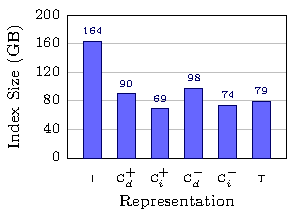
\includegraphics[scale=0.8]{plots/indexsize}
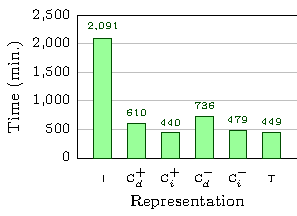
\includegraphics[scale=0.8]{plots/indextime}
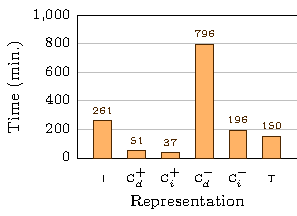
\includegraphics[scale=0.8]{plots/updatetime}
\caption{Indexing details including size (left), bulk load (mid) and version update (right) \label{fig:index}}
\end{figure}

%\begin{figure}[t]
%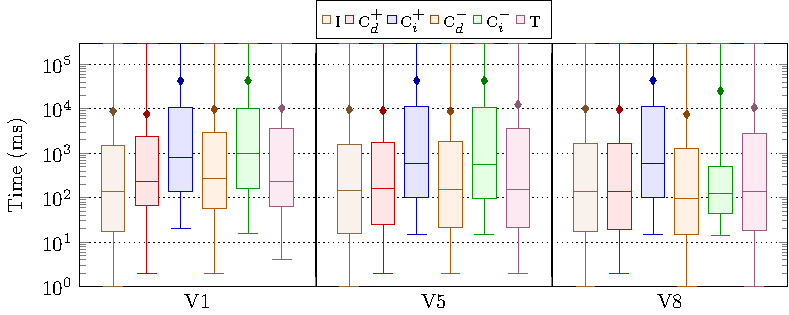
\includegraphics[scale=0.75]{plots/boxplt-svq}
%\caption{Single version query times for version 1 (left), 5 (mid) and 8 (right) \label{fig:svq}}
%\end{figure}
%
%\begin{figure}[t]
%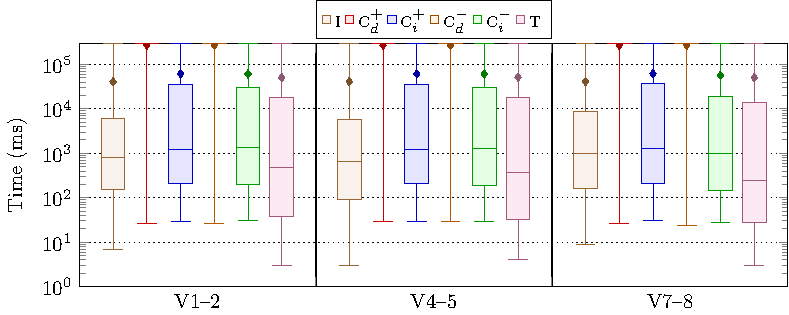
\includegraphics[scale=0.8]{plots/boxplt-dvq}
%\caption{Delta version query times for version 1--2 (left), 4--5 (mid) and 7--8 (right) \label{fig:dvq}}
%\end{figure}

\begin{figure}[t]
\centering
\begin{minipage}{.5\textwidth}
  \centering
  \includegraphics[width=\linewidth]{plots/boxplt-svq-c}
  \caption{Single version queries  \label{fig:svq}}
\end{minipage}%
\hfill
\begin{minipage}{.5\textwidth}
  \centering
  \includegraphics[width=\linewidth]{plots/boxplt-dvq-c}
  \caption{Delta version queries   \label{fig:dvq}}
\end{minipage}
\end{figure}

\section{Conclusion}

We now reflect back on our research questions: (Q1) In terms of indexing space and time, incremental builds with an initial base version (\cbpd) are best. (Q2) In general the uncompressed IC representation (\ic) offers the best query runtimes, but interval TB (\tb) is quite competitive, and even outperforms IC for delta-version queries. (Q3) Rather than there being an overall winner, we note a time--space tradeoff, where less compact representations have faster queries and more compact representations have slower queries. Interval TB (\tb) arguably strikes the best balance for space and time, though this may not hold with more versions, particularly in RDF achives where triples are often added or removed multiple times, as a quadratic number of intervals may need to be accessed.

For future work, it would be of interest to run experiments for other SPARQL engines and other RDF archive benchmarks. Also it would be interesting to run more diverse types of versioned queries, such as delta versions with larger gaps, queries returning versions as solutions, etc.; a related direction would be to consider operators from temporal logics~\cite{Pnueli77}. There are also open questions relating to more optimal/concise query rewritings, and support for paths.

In conclusion: for those who wish to host RDF archives, with different versions of an RDF graph, is SPARQL all you need? Specialised languages and systems can offer more features and consume less time and space. But with some caveats, our results suggest that query rewriting over an off-the-shelf SPARQL engine can be a solid (easy-to-deploy) option for such scenarios.

\paragraph{Online material} Please see~\cite{online} for code and queries.

\paragraph{Acknowledgements} This work was funded by Fondecyt Grant No.\ 1181896 and ANID Millennium Science Initiative Program ICN17\_002.

\bibliographystyle{abbrv}
\bibliography{paper}
\end{document}